\chapter{A kiberbiztonsági analízis megvalósítása}
% Technikai leírása a modellező eszköz architektúrájának
\section{Áttekintés}

Egy áttekintése az elemző eszköz részeinek megtekinthető a \ref{fig:04_OVERVIEW} ábrán.

\begin{figure}[!ht]
	\centering
	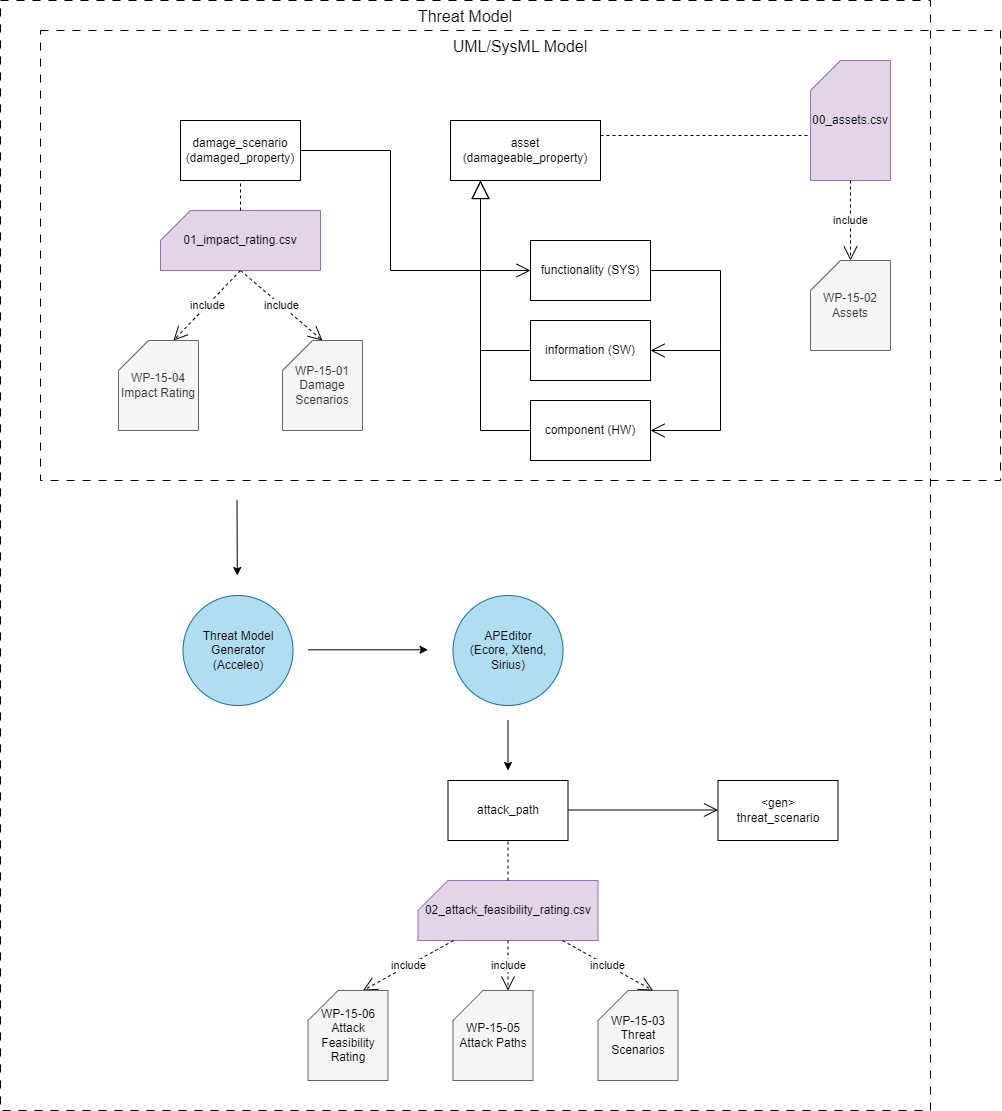
\includegraphics[width=130mm, keepaspectratio]{figures/05_overview.png}
	\caption{Megvalósítás áttekintése}
	\label{fig:05_OVERVIEW}
\end{figure}

\section{Kiberbiztonsági modell származtatása}

\subsection{Kiberbiztonsági profil}

\subsection{Fenyegetésmodell generátor}

\section{Fenyegetésmodellező eszköz}

\subsection{Metamodel}

\subsection{Fenyegetésmodell szerkesztő felület}

\subsection{Támadási fák inicializálása}

\subsection{Támadási fa szerkesztő felület}

\subsection{Dokumentum generátor}